\section{AVL Trees}
\notes{give a small introduction to the section}

\subsection{Binary Search Trees} 
\label{sec:bst}
I begin by defining a binary search tree. A binary tree is a tree data structure where each node can have no more than two children. These two children are 
called the \textit{left child} and \textit{right child} subtree. In a binary search tree, nodes are placed according to their key. The 
\textit{binary search property} states that given any node in the tree, all keys in the left child tree are smaller than that of the node, and all keys in the 
right child tree are larger than that of the node \notes{reference}. When a tree holds this property, it can be called an \textit{ordered} tree. 
This allows for lookup and insertion to be done in \notes{add complexity here} time in the worst case, as at any given node half of the tree is skipped.

\begin{figure}[!h]
  \centering
  \begin{subfigure}{.3\textwidth}
    \centering
    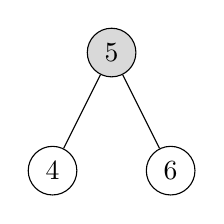
\begin{tikzpicture}
      \node[circle,draw,fill=gray!30](z){5}
      child{ node[circle,draw]{4} }
      child{
        node[circle,draw]{6} child[missing] child[missing] };
    \end{tikzpicture}
    \caption{}
    \label{fig:insert_1}
  \end{subfigure}%
  \begin{subfigure}{.3\textwidth}
    \centering
    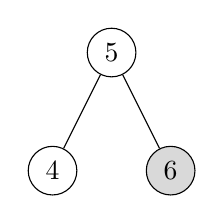
\begin{tikzpicture}
      \node[circle,draw](z){5}
      child{ node[circle, draw]{4} }
      child{
        node[circle,draw,fill=gray!30]{6} child[missing] child[missing] };
    \end{tikzpicture}
    \caption{}
    \label{fig:insert_2}
  \end{subfigure}%
  \begin{subfigure}{.3\textwidth}
    \centering
    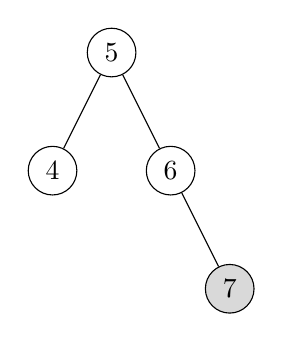
\begin{tikzpicture}
      \node[circle,draw](z){5}
      child{ node[circle, draw]{4} }
      child{
        node[circle,draw]{6} child[missing] child{node[circle,draw,fill=gray!30]{7}} };
    \end{tikzpicture}
    \caption{}
    \label{fig:insert_3}
  \end{subfigure}
  \caption{Insertion operation in a binary search tree.}
  \label{fig:insert_demo}
\end{figure}

Search, insertion and retrieval can be done recursively. Starting at the root node, the input key and the node key are compared: if the input key is smaller,
the operation is done recursively on the left subtree; if the input key is larger, then the operation is done recursively on the right subtree. Figure \ref{fig:insert_demo} shows 
a node with key 7 being inserted into a binary search tree. At \ref{fig:insert_demo}(\ref{sub@fig:insert_1}), the new node is compared to the root. As $7 > 5$, the operation continues at 
the right subtree. At \ref{fig:insert_demo}(\ref{sub@fig:insert_2}) the comparison is done again. As $7 > 6$, the operation continues at the right subtree. Because the node 6 doesn't have any children and $7 > 6$,
a new right child node is created.

\subsection{Balance and rotation}
An AVL tree is based on a binary search tree, with one very important distinction - it is \textit{balanced}. To define what it means for a tree to be balanced, I will first
define what the \textit{height} of a tree is. \notes{get concrete definition of tree height}. Balance is reliant on this definition - an AVL tree is only balanced when the 
heights of any given left and right child subtrees does not differ by more than one \cite{avl:original}. By keeping balance, the structure ensures that there is a high ratio between the number of 
nodes in the tree and the height. This allows for retrieval and search operations to be done in $O(\log n)$ time in the worst case, with $n$ being the amount of nodes in a tree \cite{avl:computer}.

During the insertion operation, the tree can become imbalanced, which can be mitigated
with either a right rotation or a left rotation. 